\documentclass[10pt,a4paper]{article}
\usepackage[utf8]{inputenc}
\usepackage[spanish]{babel}
\usepackage{textcomp}
\usepackage{graphicx}
\graphicspath{ {./images/} {./images2/} }
\usepackage[left=2cm,right=2cm,top=3cm,bottom=2cm]{geometry}
\author{José Isaac Zeledón Jiménez, Jonathan Estrada Vargas}
\title{Proyecto 0}
\begin{document}
\begin{titlepage}
\begin{center}
\begin{large}
UNIVERSIDAD NACIONAL\\
COSTA RICA \\
\end{large}
\vspace*{1cm}
\begin{large}
Facultad de Ciencias Exactas y Naturales
\end{large} 
\vspace*{1.8cm}\\
Asignatura:\\
\vspace*{2mm}
\begin{large}
Paradigmas de Programación\\
\end{large}
\vspace*{12mm}
\begin{large}
\textbf{PROYECTO 0: 
PROGRAMACIÓN GÉNETICA
}\\
\end{large}
\vspace*{1.8cm}
Profesor:\\
\vspace*{5mm}
\begin{large}
Eddy Miguel Ramírez\\
\end{large}
\vspace*{1.8cm}
Estudiantes: \\
\vspace*{5mm}
\begin{large}
Andrés Jiménez Elizondo\\
Jonathan Estrada Vargas\\
José Isaac Zeledón Jiménez\\
\end{large}
\vspace*{1.8cm}
II CICLO\\
\vspace*{1.8cm}
2019
\end{center}
\end{titlepage}
\tableofcontents
\pagebreak
\section{Introducción}
\bigskip
\bigskip 
\bigskip 
\bigskip 
	Este proyecto que tiene el objetivo, de que, el equipo de desarrollo conozca el paradigma de programación funcional, además de conocer un nuevos conceptos que son los algoritmos genéticos.\\\\
	El profesor presentó el problema de encontrar utilizando las técnicas de algoritmos géneticos, las funciones que cumplieran que al ser evaluadas con distintos valores de x y se acercaran lo máximo posible a los z dados en la tripletas de que el profesor nos facilitó, estas tripletas, son puntos por los que la función original pasa, de forma que mediante la técnicas de algoritmos genéticos se intenta llegar aproimar a esa función.\\\\
	Las técnicas de algoritmos genéticos utilizadas son las básicas consideradas en este tipo de programación. El problema se enfretó de la manera que se le llamaría por la teoría de algoritmos genéticos, generacional con elitismo. El elitismo es la técnica en la que el mejor individuo de la población pasa a la siguiente generación.\\\\
	También en el documento se describirán los distintos problemas enfrentó durante el desarrollo del proyecto, las que comúnmente  están relacionadas con el paradigma, ya que la formación del equipo de desarrollo se da en paradigmas en los que es común el uso de variables y constantes, lo que no es común utilizar en el paradigma funcional, además de que el también el lenguaje de programación que se utilizó puede llegar a ser complicado si todavía no se posee el $"pensamiento$  $funcional"$ que el profesor recomendó desarrollar para el uso de este lenguaje de programación.\\\\
	El lenguaje de programción utilizado en el desarrollo de este proyecto fue Scheme, el cuál es un subconjunto de el lenguaje de programación LISP; segundo lenguaje de programación (1958); Scheme fue desarrollado en el MIT (Massachusetts Institute of Technology) , en este lenguaje se desarrolló la mayoría de las funciones de algoritmos genéticos, además fue necesario la utilización de ciertas funciones de racket para la tarea de graficar los de las funciones y los puntos a los que se debía aproximar.\\\\
	Se dará una especificaión de la solución al problema, donde se describe la forma en la que el equipo de desarrollo atacó la elaboración de las funciones, ya que lo que pasa con este proyecto es que al ser de algoritmos genéticos la solución a la que se desea llegar se logra al poner el programa a correr durante un tiempo considerable para que la aproximación se dé de la mejor manera.\\ 
\pagebreak
\section{Descripción del Problema}
 El problema consiste en que para funciones de 3 dimesiones  $"adivinar"$ la función a partir de puntos que interseca es
difícil, así que para esto se debe de hacer un proceso automatizado en el que de forma aleatoria se creen funciones para evaluarlas con respecto a los puntos que interseca y de ahí se elija a las mejores para hacer una aproximación más precisa, esto por medio del cruce y la creación de generaciones de individuos.\\\\
Para esto se puede utilizar varios recursos redes neuronales, o como en esta ocasión se esta utilizando los algortimos genéticos, lo que está basado en la selección natural de Charles Darwin que favorece a el individuo con mejores características. Con esta premisa se puede explicar que ciertos de los conceptos de algoritmos genéticos. Los mismos son los siguinetes, individuo, poblacion, función fitness, cruce, generaciones y elitismo. \\\\
\begin{itemize}
\item Individuo: es una estructura de datos, en este caso particular árboles binarios de expresión. \\
\item Población: un conjunto de individuos.\\
\item Función Fitness: es un función que $"califica"$ a los individuos de la población y conforme a sus características les otorga mejor o peor calificación. \\
\item Cruce: es el proceso en el cuál los individuos de una población se cruzan para generar una nueva generación, este cruce está dado de forma aleatoria entre los miembros de la población de la población eso sí con una técnica de selección la cual favorece a los mejor calificación en la función fitness.\\
\item Generaciones: son el producto de los cruces de las población, entre más generaciones haya se espera que sea más precisa la aproximación a la respuesta correcta.\\
\item Elitismo: es una técnica utilizada, cuando se resuelve un problema con la metodología generacional, en la cual se asegura la sobrevivencia del mejor individuo haciendo que esté en la siguiente generación para así no perder la buenas caracteristicas del mismo en la siguiente generación. \\
\end{itemize}
Con lo anterior se puede apreciar de una mejor manera el rumbo por el cual el problema se iba resolver. 
Se puede apreciar como el problema se vale de la técnicas de selección natural para la escogencia del mejor individuo de la población ya que la implentación de la función fitness es crucial y donde tenemos que garantizar que la evaluación dada, no va llegar a una situación en la que se quede estancada y las generaciones no se acerquen a el punto esperado.\\\\
Otro detalle que se debe de considerar es la escongencia del tamaño de la población ya que como el profesor explicaba, si la población es muy pequeña existe poco pool genético, lo que genera endogamia, y por el contrario si se da que la población es  muy grande lo que pasa es los individuos de mejores características, si son pocos, se ven opacados porque la población es tan grande que pasan desapercibidos entre toda la población. Por lo que hay que encontrar un tamaño correcto de población, esto es algo que el equipo de desarrollador no sabe, ya que no se encontró una métrica para la escogencia del tamaño de la población.\\\
\pagebreak
\section{Especificacion de la solución}
 Este apartado se describirá, la implementación de algunos  de los códigos que generan el programa, para encontrar la solución.\\
Por recomendación del profesor, la solución se separó en pequeñas funciones, que cumplen con una tarea específica.\\\\
En la especificación del proyecto, se dice que los individuos de la población (árboles binarios de expresión) y que los operadores que pueden llegar a formar la expresiones son los siguientes: $(+$ $-$ $/$ $*$ $expt$ $log)$. Por lo que siguiente función es para escoger uno de los operadores de forma aleatoria.  
\begin{verbatim}
(define random-op
  (lambda ()
  (list-ref '(+ - / * expt log) (random 6))))
\end{verbatim}
 La siguiente función es la que se utiliza para evaluar los arboles binarios de expresión, esto haciendo del uso del eval de scheme. 
 \begin{verbatim}
 (define evalua
  (lambda (L a b)
    (eval (list (cons 'lambda (cons '(x y) (list L))) a b))))
 \end{verbatim}
 La función que sigue nos ofrece de forma aleatoria el retorno de los valores aleatorios de x y o un número, que fue utilizado en la función de crear el árbol.
 \begin{verbatim}
 (define xynum
  (lambda ()
    (cond ((= (random 2) 0) 'x)
          ((= (random 2) 1)  'y)
          (else (random 10)))))
\end{verbatim}
 La función de que sigue es la que de forma aleatoria se define si el elemento es una hoja. 
 \begin{verbatim}
 (define es-hoja?
  (lambda ()
    (< (random 100) 50 )))
 \end{verbatim}
 Las siguientes funciones son las que se utilizaron para generar el árbol de expresión.
 \begin{verbatim}
(define arbolaleatorio
	(lambda ()
	 (list(random-op) (arbol2) (arbol2))))
\end{verbatim}
\begin{verbatim}
(define arbol2
	(lambda ()
		(cond ((es-hoja?) (xynum))
		(else (arbolaleatorio)))))
\end{verbatim}  
La siguiente función es la que crea la población inicial con la que se inicia la evaluación de individuos para intentar llegar a $"adivinar"$ la función.
\begin{verbatim}
(define inicial
  (lambda (n)
    (cond ((zero? n) '())
          (else
          (cons(arbolaleatorio) (poblacion (- n 1)))))))
\end{verbatim}
Corriendo la f2 se logró los sigueintes resultados con un número de 9 generaciones y una población de 20 indiciduos se encontró los siguientes resultados.\\
\begin{center}
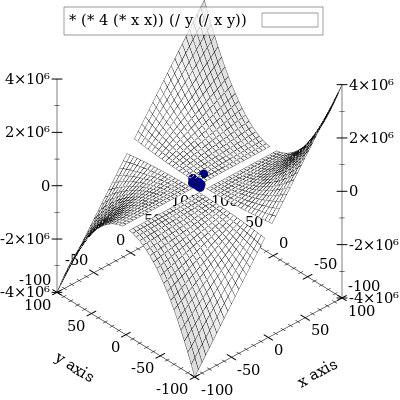
\includegraphics[width=5cm, height=5cm]{f1-1}
\end{center}
\begin{center}
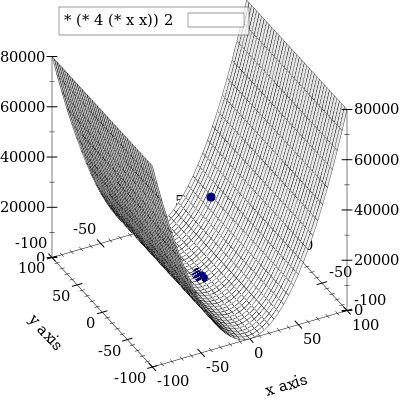
\includegraphics[width=5cm, height=5cm]{f1-2}
\end{center}
\begin{center}
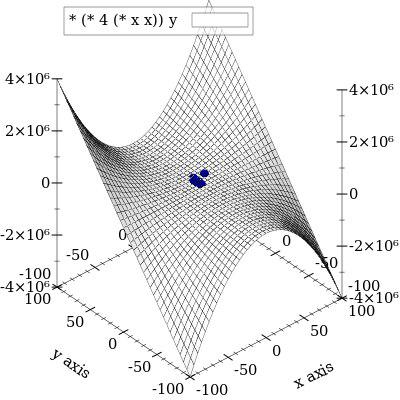
\includegraphics[width=5cm, height=5cm]{f1-3}
\end{center}
\begin{center}
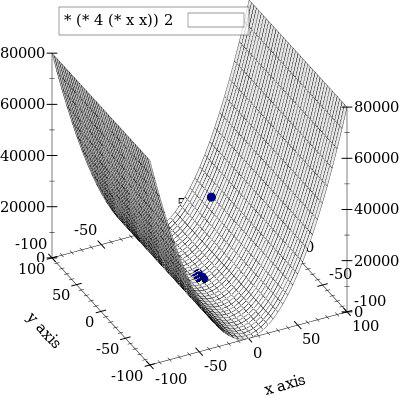
\includegraphics[width=5cm, height=5cm]{f1-4}
\end{center}
\begin{center}
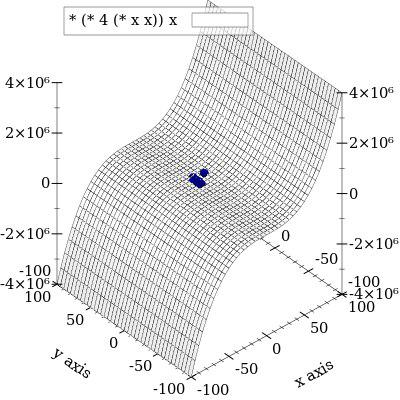
\includegraphics[width=5cm, height=5cm]{f1-5}
\end{center}
\begin{center}
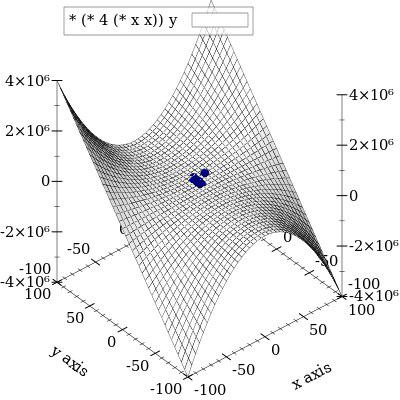
\includegraphics[width=5cm, height=5cm]{f1-6}
\end{center}
\begin{center}
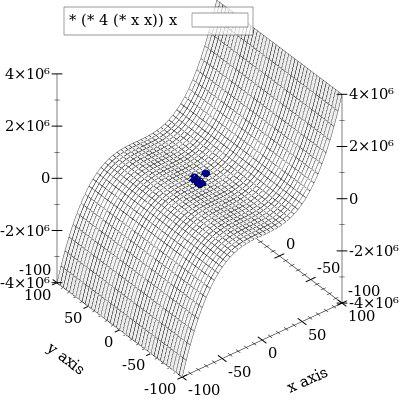
\includegraphics[width=5cm, height=5cm]{f1-7}
\end{center}
\begin{center}
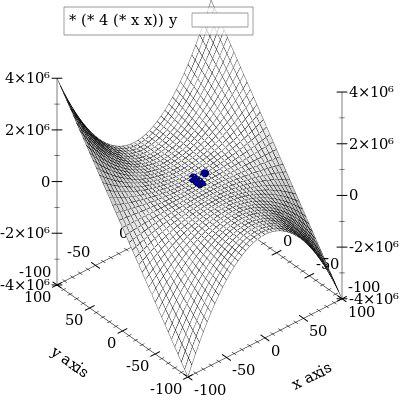
\includegraphics[width=5cm, height=5cm]{f1-8}
\end{center}
\begin{center}
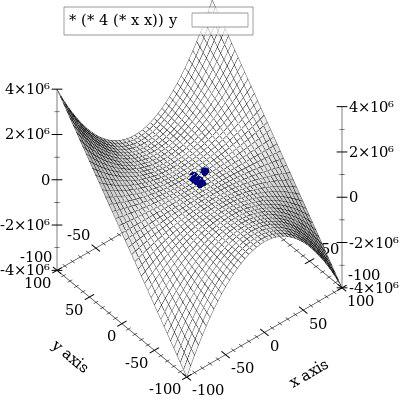
\includegraphics[width=5cm, height=5cm]{f1-9}
\end{center}
Corriendo la f3 se logró los sigueintes resultados con un número de 20 generaciones y una población de 20 individuos se encontró los sigueintes resultados.\\
\begin{center}
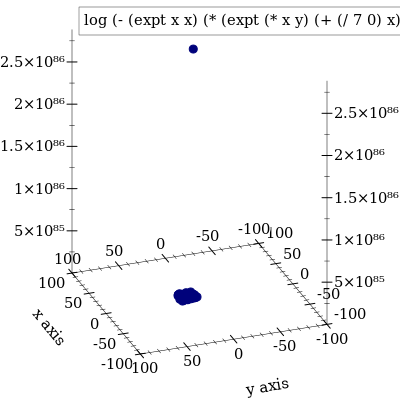
\includegraphics[width=5cm, height=5cm]{19}
\end{center}
En ciertas ocasiones se presentaba el problema en el que no se graficaba la función.\\
\begin{center}
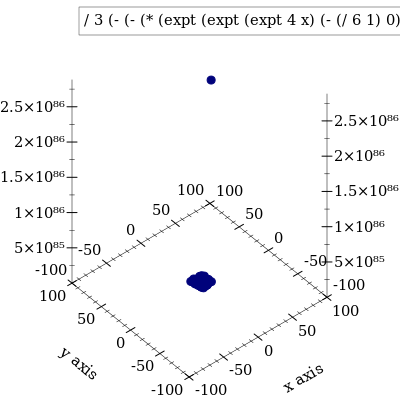
\includegraphics[width=5cm, height=5cm]{18}
\end{center}
Pero podemos apreciar que en la función siguiente ya es visible la grafica de la función
\begin{center}
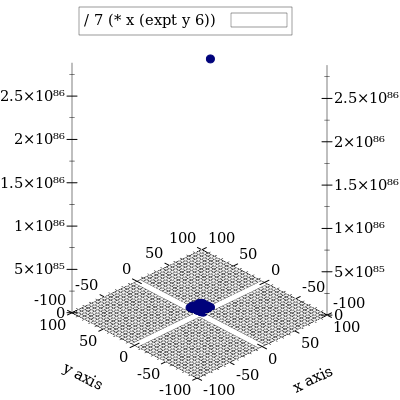
\includegraphics[width=5cm, height=5cm]{17}
\end{center}
\begin{center}
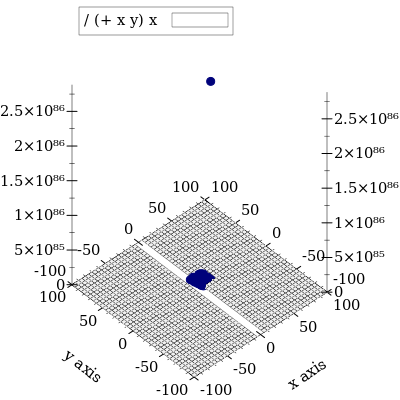
\includegraphics[width=5cm, height=5cm]{16}
\end{center}
\begin{center}
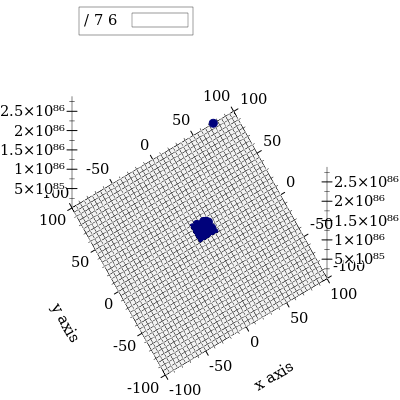
\includegraphics[width=5cm, height=5cm]{15}
\end{center}
\begin{center}
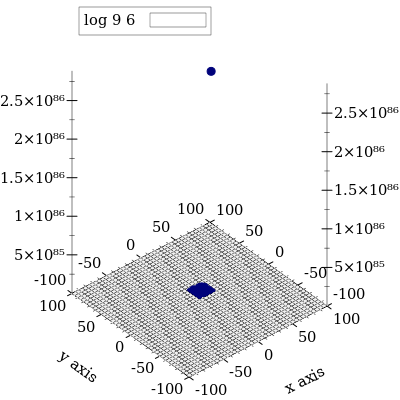
\includegraphics[width=5cm, height=5cm]{14}
\end{center}
\begin{center}
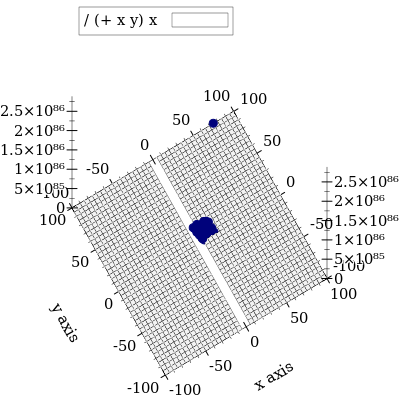
\includegraphics[width=5cm, height=5cm]{13}
\begin{center}
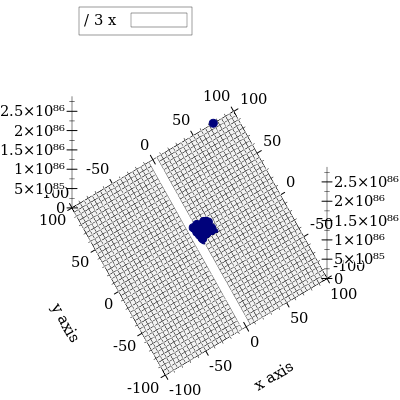
\includegraphics[width=5cm, height=5cm]{12}
\end{center}
\begin{center}
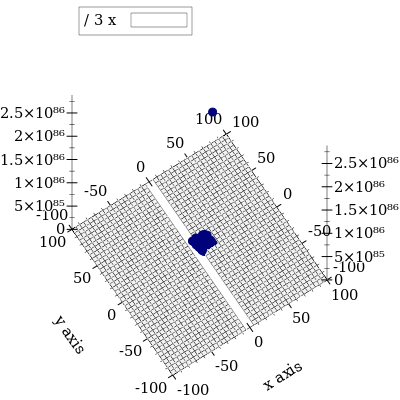
\includegraphics[width=5cm, height=5cm]{11}
\end{center}
En cada una de las imágenes se puede apreciar a el mejor individuo de cada generación.\\
\begin{center}
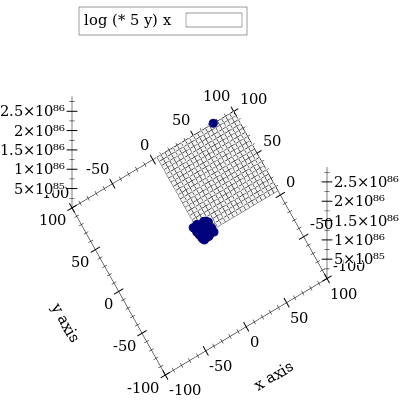
\includegraphics[width=5cm, height=5cm]{10}
\end{center}
\begin{center}
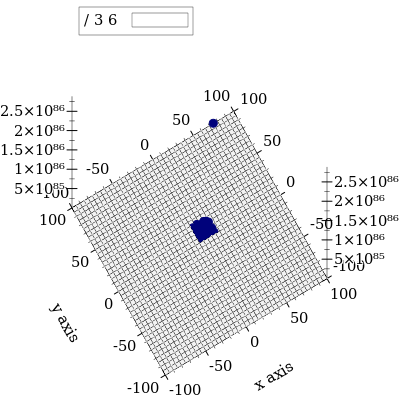
\includegraphics[width=5cm, height=5cm]{9}
\end{center}
\begin{center}
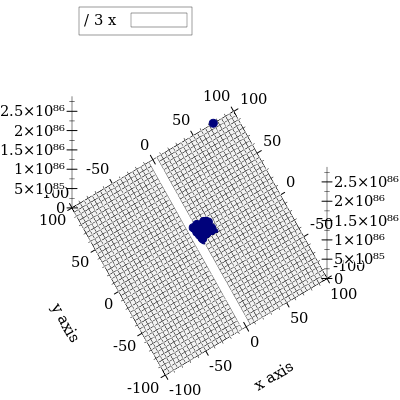
\includegraphics[width=5cm, height=5cm]{8}
\end{center}
\begin{center}
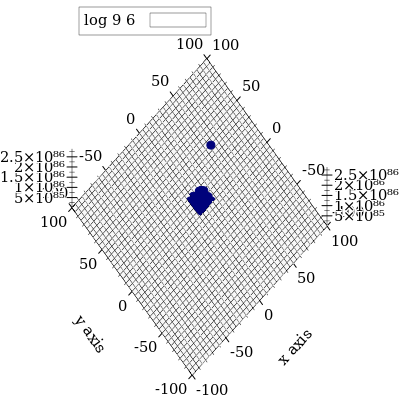
\includegraphics[width=5cm, height=5cm]{7}
\end{center}
\begin{center}
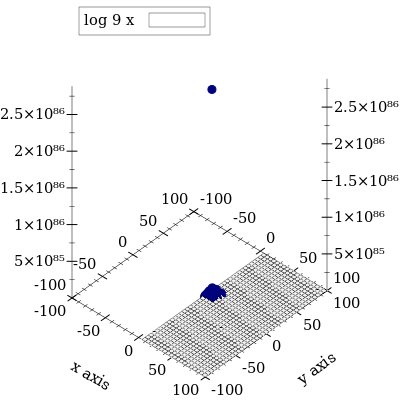
\includegraphics[width=5cm, height=5cm]{6}
\end{center}
\begin{center}
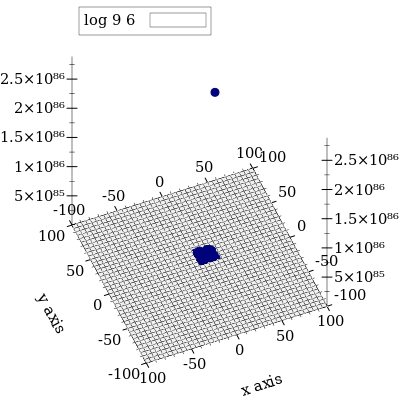
\includegraphics[width=5cm, height=5cm]{5}
\end{center}
\begin{center}
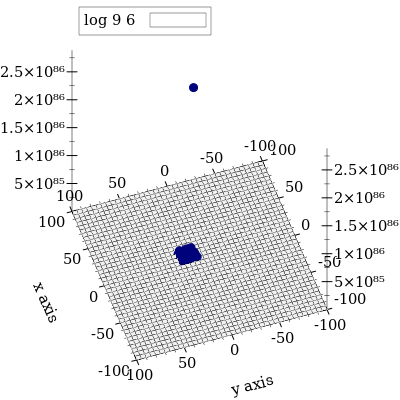
\includegraphics[width=5cm, height=5cm]{4}
\end{center}
\begin{center}
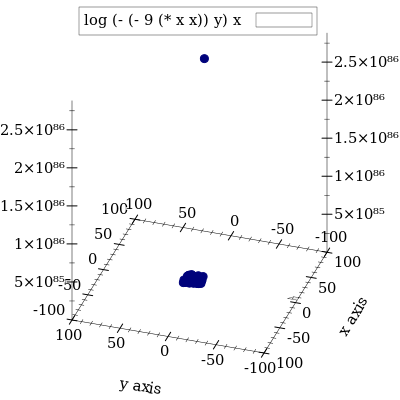
\includegraphics[width=5cm, height=5cm]{3}
\end{center}
\begin{center}
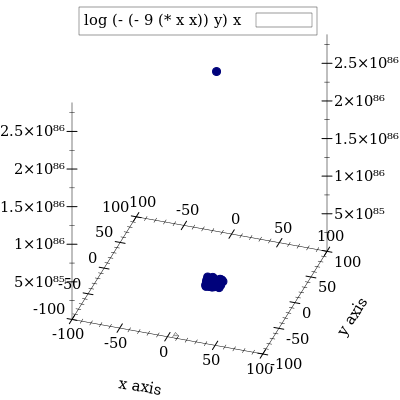
\includegraphics[width=5cm, height=5cm]{2}
\end{center}
\begin{center}
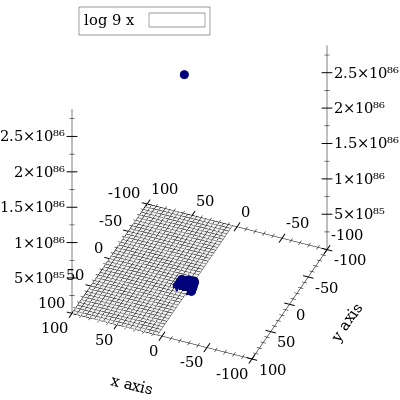
\includegraphics[width=5cm, height=5cm]{1}
\end{center}
\end{center}
\pagebreak
\section{Problemas encontrados}
Durante el desarrollo de un proyecto nunca se está libre de dificultades algunas de las que se encontró en el desarrollo de este fue el paradigma de programación, ya que ciertas implementaciones eran difíciles de pensar en el paradigma funcional, ya que se está acostumbrado a utilizar el paradigma orientado a objetos. \\
La implementación de ciertos conceptos de algortimos genéticos
como el individuo (estructuras de datos), y la seleción aleatoria de los individuos para el cruce de los mismos.\\
Además de la implementación de la función fitness la cual se evalua sobre los individuos y que sin ella la evolución de las generaciones no sería posible.\\
Estos problemas de implementación encontrados dificultó el tiempo para dedicar a que los algoritmos genéticos corrieran y ver la evolución de la generaciones con respecto al tiempo.\\
\section{Conclusiones}
	Con respecto a la evolución de las generaciones con conforme a las funciones se posee una opinión reservada ya que debido a limitaciones de hardware se debió de limitar la cantidad de las generaciones ya que sino la visualización de la gráficas no era algo posible, además de que el programa dejaba de funcionar al correr durante mucho tiempo.\\
	En general podemos decir que el aprendizaje sobre los conceptos y aplicaciones de los algoritmos genéticos es bueno y además se puede envidenciar que los intengrantes del equipo desarrollador nos poseían conocimiento alguno en lo que a este tema se refiere.\\
	Se puede afirmar que luego se pondrá a correr el programa para ver de que forma evolucionan las funciones resultantes de los cruces, además de si existe un estancamiento en lo que se refiere a la funcion de evaluación concierne.\\
\end{document}
\end{document}
